%Template credit: Jan-Willem Steeb, NRAO

\documentclass[12pt,a4paper]{article}

\usepackage{graphics,graphicx}
\usepackage[%
    font={small,sf},
    labelfont=bf,
    format=hang,    
    format=plain,
    margin=0pt,
    width=0.8\textwidth,
]{caption}
\usepackage[list=true]{subcaption}
\usepackage{amsmath}
\usepackage{amssymb}
\usepackage{bm}
\usepackage{listings}
\usepackage{hyperref}
\usepackage{lmodern}  
\usepackage{amsmath}  
\usepackage{xcolor}   
\lstset{
  basicstyle=\ttfamily,
  columns=fullflexible,
  frame=single,
  breaklines=true,
  postbreak=\mbox{\textcolor{red}{$\hookrightarrow$}\space},
}

\textheight=247mm
\textwidth=180mm
\topmargin=-7mm
\oddsidemargin=-10mm
\evensidemargin=-10mm
\parindent 10pt

%%%%%%%%%%%%%%%%%%%%%
%%%%% Custom Commands %%%%
%%%%%%%%%%%%%%%%%%%%%
\newcommand{\vb}[1]{\text{\textbf{#1}}} %make non special characters bold in math mode, used for vectors and matrices
\newcommand{\n}[1]{\text{{#1}}} %removes math styling, useful for subscripts

%Mathematic Functions
\DeclareMathOperator*{\argmax}{arg\,max}
\DeclareMathOperator*{\argmin}{arg\,min}
\DeclareMathOperator*{\mmid}{mid}
\DeclareMathOperator*{\at}{arctan2}

%%%%%%%%%%%%%%%%%%%%%
%%%%% Start of document %%%%% 
%%%%%%%%%%%%%%%%%%%%%

\begin{document}
\pagestyle{plain}
\pagenumbering{arabic}
 
%%%%%%%%%%%%%
%%%%% Title  %%%%%
%%%%%%%%%%%%%%

\begin{center}
{\Large{\bf{  GBO python  \\  }}} 

\end{center}
\bigskip

\centerline{Peter Teuben (University of Maryland, USA)}

\centerline{Version 0.2 - \today}
\bigskip

\section{Overview}

The GBT/GBO single dish processing software is reviewed in light of
a more coherent workflow using python on the top level, and abandoning the
IDL licensed software.\footnote{weather info is also needed in some
  calibration procedures, making it still hard to work offsite}

The current data formats is SDFITS, and will continue to be used.

We will however take this opportunity to review the whole workflow of
single dish data processing from the astronomers' point of view, by
comparing functionality offered in other packages such as {\tt comb},
{\tt SPECX}, and {\tt CLASS}. The predecessors of {\tt GBTIDL} are
{\tt DISH} (under AIPS++) and before that {\tt uniPOPS}. They are largely
functionally equivalent, just using other command processors. At the
current time (2019 as we write this), python is the most likely
candidate for a data processing package dealing with single dish
data. Given usage of jupyter notebooks, it would also be nice if any
new efforts could make use of this.

\begin{figure}[h]
\centering
  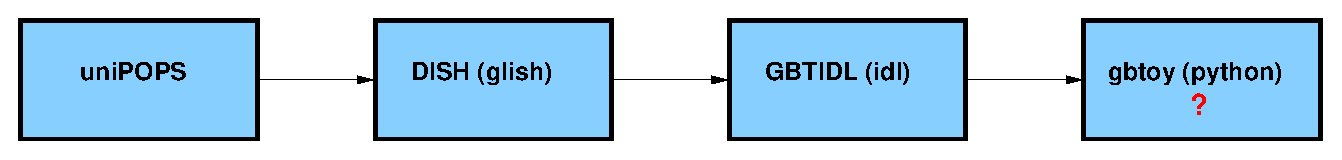
\includegraphics[width=\textwidth]{fig1.eps}
\caption{\label{fig1} Evolution of the GBT analysis software.}
\end{figure}

\section{Functionality}

What is the functionality we would want from a Single Dish Data Reduction
package? 

\begin{itemize}

\item Deal with spectra on an individual (or group?) basis
  \begin{itemize}
\item Visualize spectra, a versatile interactive plotting tool is needed
  that can handle overlaying fits and/or other spectra
\item Calibrate spectra (Freq, Pos, Nod)

\item Flagging/Masking data

\item Edit header (e.g. to fix problems)  

\item Fit models to spectra


  \end{itemize}


\item good batch system for pipeline and/or scripts to define a workflow on one spectrum
  and then apply it to all
  

  
\item Organize spectra by properties such as RA, DEC (for gridding) - is there even anything else?

\item Gridding spectra in RA,DEC or GLAT,GLON, even in AZ,EL for debugging?

\item Work with lag spectra?

\item Does OTF have special needs?

\item integrate well with a python eco-system. Many users are now familiar with
  python, numpy etc.  If the code allows us to get and set numpy arrays,
  that's a gain. It should also be usable via a the classic ``import''
  mechanism, and expected to work well with packages such as astropy and jupyter
  notebooks. Use of widgets would be interesting too, but that's very notebook
  specific.
\end{itemize}


\section{Existing GBT code}

We are faced with 3 existing packages: {\tt GBTIDL}, {\tt gbt-pipeline} and
{\tt gbtgridder}, of which the latter two are already in python. There is also
a derived product, {\tt gbtpipe}, written by Erik Rosolowsky. All codes are
publicly available. Some code overlap has been noticed. The pulsar timing observations are
in a completely different category, and will be ``ignored'' for the
moment until we understand what to do with them. Another point to keep in mind is that
the ``dialects'' that seem to exist in the SDFITS format are specific to the backend.

Nomenclature of SD observations ({\it as found in one of the GBT manuals}):

\begin{itemize}
  \item[{\bf region}]  : over many days and possibly RA/DEC
  \item[{\bf session}] : same 'day' continguous in time
  \item[{\bf block}]   : observation unit
  \item[{\bf scan}]    : integrations that belong together (few mins)
  \item[{\bf integration}] : integration of a specific state (pointing, band, polarizations, ...)
\end{itemize}   


In addition there are several ways how to calibrate SD spectra, broadly separated
into position and frequency switching. Calibration also depends on the instrument used,
and the SDFITS ``dialect'' will play a role in this.

\begin{itemize}
\item
nodding:    a mirror like device make it look at a different "blank" sky
nodding secondary. or are there other nodding options?
\item
position:   telescope physically looks at a different "blank" sky?
\item
frequency:  use a nearby part of spectrum to be able to baseline subtract
\end{itemize}

OTF (e.g. \cite{2007AA...474..679M})
would scan over the source far enough out that the ``off'' positions are reached at
the edges of the scans.

\section{GBTIDL}

As a reminder, here is a example\footnote{taken from the GBTIDL Users' Guide}
where you get a quick look and feel of the command line interface in GBTIDL:

\begin{lstlisting}[language=bash]
% gbtidl                         ; Start GBTIDL from the unix prompt

GBTIDL -> filein, 'myraw.fits'   ; Specify an input SDFITS file
GBTIDL -> summary                ; Give a summary of the scans in the opened data file
GBTIDL -> getfs, 9               ; Retrieve, calibrate, and plot a frequency switched  
                                 ;  spectrum (other observing modes use different commands)

GBTIDL -> setregion              ; Set region used to determine baseline
GBTIDL -> nfit,2                 ; Specify that a 2nd order baseline will be used
GBTIDL -> baseline               ; Fit and subtract a baseline

GBTIDL -> fitgauss               ; Fit a Gaussian profile to the plotted spectrum.  The mouse
                                 ;  is used to set initial guesses

GBTIDL -> stats                  ; For the displayed spectrum, show statistics such as
                                 ; the RMS, maximum and minimum x and y values
GBTIDL -> print_ps               ; Write the current spectrum to a postscript file

GBTIDL -> fileout, 'mydata.fits' ; Specify the output file name for saved data
GBTIDL -> keep                   ; Save the spectrum currently displayed
		    
GBTIDL -> exit                   ; Exit GBTIDL

\end{lstlisting}

\subsection{Conversion to python?}

GBTIDL can be 'converted' to python in several ways:

\begin{enumerate}
\item
  keep the function names and functionality the same as much as possible,
    but use {\tt pyspeckit} under the hood
\item
  same as 1), but literally  translating IDL to python. A lot more work.
  Functionally the same as  was done uniPOPS to dish to gbtidl it seems.
  This would add just one more in the chain.
\item
  using pyspeckit natively. raw python power. This is possibly a harder way for
  existing users to switch to and accept. Might as well force CLASS on them.
\item
  bringing the sdfits interfaces that gbt-pipeline uses into the loop.
probably not useful to 1) , but could be useful for 2)

\end{enumerate}

Either way, the peculiar graphics display that GBTIDL is using should
be investigated if pure matplotlib has this functionality, or do we
need an embedded wxPython ot QtPython interface around it (or another
GUI wrapper).  \url{https://docs.python.org/3/faq/gui.html}


\subsection{Data}

\subsection{The SDFITS standard}

Although there is an SDFITS standard, there are some clear dialect issues. For example,
the pyspeckit 3C286.fits file does not work in GBTIDL. Also, the 3 standard examples
from GBTIDL do not work in pyspeckit, because newer header items (e.g. TRGTLONG) are
absent, because pyspeckit assumed them to be present. They are GBT specific.
The number of GBT specific header elements has been steadily increasing. The 2005 data
have about 46, there are 79 in the 2016 GBT EDGE data.

The {\tt sdheader} script tries to assembles this knowledge.

\subsection{Possible Test Cases}

We will need some standard datasets that have known answers. They probably will come in SDFITS format.

We have the following options:

\begin{enumerate}

\item
  The 3 examples in the users' guide (ngc5291.fits , W3OH.fits, IC1481.fits) [all 2005]
\item
  The 2 examples in the SDFITS standards page (TREG\_091209.cal.acs.fits [2009], Parkes\_GASS.fits [2010?])
\item
  The example in the pyspeckit packate (3C286.fits [2012])
\item  
  The 2nd example in the pyspeckit package, AGBT11B\_029\_01.raw.acs.fits, absent from archives , but I found a calibAGBT02C\_023\_03.fits [2005]
\item
  M81/M82 2003 data as described on\newline
  \url{https://safe.nrao.edu/wiki/bin/view/GB/Data/M81ExampleExectution}
\item
  EDGE survey data via Tony Wong [2016]
\item
  ARGUS data?
\end{enumerate}

There appear to be some SDFITS ``dialect'' issues between these files that need to be understood.
{\tt pyspeckit} deals with very little variation.

\section{Other Software}

Here we describe related software packages which could have an impact on the design:

\subsection{comb}

Turns out Alberto has also used this, but Marc Pound is our local resident expert.

Before we list the famous two-letter commands in {\tt comb}, first some nomenclature within {\tt comb}:

\begin{itemize}
  
\item A {\bf stack} is a spectrum for local processing (as opposed to a
  {\bf scan} which is the unprocessed but typically calibrated spectrum).
  In comb, stacks 1-3 are in memory and stacks 4-N are disk storage.
  
\item  
  The {\bf use array} is the bitmask of channels to use when subtracting a
  baseline (there will forever be the confusion of what a mask means: use it
  or not use it, and does this apply to where the signal is, or where there
  is no signal and the baseline needs to be fitted). Not unlike the difference
  between masks in python and casa.
  
\end{itemize}

Here's the list of COMB commands.  They can be broadly put in two categories:
system functionality which the python eco-system will solve for us (e.g. {\tt c},
{\tt cm}, {\tt cp}, {\tt do} etc.) and which are functional tools to operate
on spectra (e.g. {\tt ad}) which we'll need to check on how GBTIDL does this.

\footnotesize\begin{verbatim}
ad - Add scans to stack2                          check
af - Attach a FITS file to an image               check
bc - Designate bad channels                       check
c - Calculate something                      Py
ca - Calculate values from stacks                 check
cc - Change center channel                        check
cm - Space-space Contour Map                 Pl
co - Combine two stacks, result in 1 & 2          check
cp - Contour Plot an image                   Pl
cr - Cursor read                             Pl
cv - Convolve stack 1 with stack 3                check
da - Define an area of an image                   check
dm - Define macro                            Py
do - Loop through a command string           Py ?
dv - Declare user Variables                  Py 
e - Execute a shell command                  Py
el - Eliminate bad chans in stack 1.
em - Empty a stack
fl - Flag location on graph
fo - Fold freq switched data in stack 1
ft - Fourier operations on baseline
gf - Fit a gaussian function to part of a spectrum
gm - Graphics Manipulation
gt - Put scan in st 1
hc - Make a Hard copy of the current screen
im - Image manipulate
in - Integrate part of a spectrum
is - Interpolate a spectrun for a given position
lc - List commands
li - Fit and remove a polynomial baseline
lk - Look at where stacks are on the sky
me - Map data Extraction
nf - Switch data files
ns - Name stacks directory
op - Set options
p - Print something
pa - Pause in execution
pd - Print data
pf - Fit a parabola to part of a spectrum
ph - Print in hms format
pl - Plot stack 1
pr - Printf to standard output or a string variable
q - Exit comb
rc - Define relative coordinate system
ri - Redirect command input from a file or string
rm - Calculate rms and ssb noise figure for stack 1
ro - Redirect output to a file or string variable
rs - Rescale and add constant to stack 1
rt - Retrieve stack
sc - Scanf from a file, stdin, or a string variable
sl - Make a slice through an image
sp - Make a scatter plot comparing two images
sq - Squish - increase or decrease chan width
st - Store stack
th - Temperature Histogram
tp - Total power - average chans in stack1 weighted by cal in stack3
uf - Execute a user function on stack 1
up - Update a stacks directory
us - Change use array
v - Compute value for map
vc - Velocity Space Contour Plot
vm - Calculate Virial Mass
wc - Write data Cube
wf - Write an image to a FITS file
wr - Write scan back onto file
wu - What is up (Plot source positions in az and el)
xf - Transfer stacks to directory 2 after making them unique (1/position)

\end{verbatim}
\normalsize

\subsection{SpecX}

This is a pretty old package, lives within Starlink? Was used on JCMT. It's
basis is  RPN arithmetic and a stack. It seems to have a rich interactive
plotting interface. I've only found VMS based manuals,
but internally has its own command language.

Some example commands:
\footnotesize\begin{verbatim}

read-spectrum \1\27

open-fits-file
write-fits-spectrum
close-fits-file

multiply-spectrum 5.1 ; offset-spectrum 2; new-plot

clip-spectrum
drop-channels
invert-spectrum
remove-spikes
set-channels
truncate-spectrum

remove-linear-baseline


\end{verbatim}
\normalsize

\subsection{UniPOPS}
the pre-historic program on which everything (DISH, GBTIDL) seems to be based
\url{https://www.cv.nrao.edu/unipops/}


\subsection{DISH}
DISH was based on uniPOPS. ADASS 1999(?) has several papers dedicated to dish:
\cite{2000ASPC..216..498G},
\cite{2000ASPC..216..494G}, and 
\cite{2000ASPC..216..243G}.

(AIPS++ and glish):  https://safe.nrao.edu/wiki/bin/view/GB/Data/DishUsersGuideForGBT

Note that GBTIDL derived all the functionality from DISH, which in itself was derived from UniPOPS,
but DISH has a gridder.

       scan  - integrations 

\subsection{CASA/sd}
  there is an SD package, which originated with the Nobeyama 45m\newline
  \url{https://casa.nrao.edu/casadocs/casa-5.4.1/single-dish-calibration/single-dish-data-calibration-and-reduction}

\subsection{CLASS}

We have several experts locally: Alberto, Miguel/Andy, Maitraiyee
  
 https://www.iram.fr/IRAMFR/ARC/documents/filler/casa-gildas.pdf
      http://www.iram.fr/IRAMFR/GILDAS/
      and their new python interfaces:

\subsection{NOD3}

Seems to be used at Effelsberg.

\subsection{AO IDL}

Arecibo has their own IDL based data reduction package.

Some info on \url{http://www.naic.edu/~astro/data/data_formats/idl/index.shtml}

\section{Other Telescopes}

Here's a brief inventory of what software is used at other SD telescopes
\begin{itemize}
  \item ALMA/TP 12m: CASA
  \item APEX 12m: CLASS
  \item Arecibo 305m: AO IDL
  \item Effelsberg 100m:  NOD3, but also new python things (Winkel)
  \item FAST 500m:
  \item GBT 110m:  gbtidl
  \item IRAM 30m: CLASS
  \item JCMT 15m:
  \item LMT 50m:
  \item Lovelll 76m:
  \item Nobeyama 45m:   casa?
  \item Parkes 64m:
  \item SRT 64m: GILDAS, SDI, SCUBE, 
\end{itemize}       
       

\section{gbtoy}       

GBTOY is a toy model for GBTIDL, pythonizing their familiar commands
(going back 3 different software packages).

In this version we use pyspeckit (+astropy) under the hood, since it
knows how to handle SDFITS files and has a graphics
interface. Currently this means only nodding reduction is supported,
no frequency switching yet (not sure about position switching).

The goal in this "toy" version is to explore how a pythonic GBTIDL would
look and feel and get user feedback before we continue.

Another way is to base the code more on pyspeckit, or really extend
pyspeckit to make it cover the known GBTIDL cases.  Two GBT examples
exist in pyspeckit-tests, and only 3C286 sort of works now, while
jd\_test with AGBT11B\_029\_01.raw.acs.fits currently lacks the data.
Example test:  \url{https://github.com/pyspeckit/pyspeckit-tests/blob/master/test_3c286.py}

A third way is to inspect the gbt-pipeline code. It has methods to
read SDFITS file, but lacks the interactive parts of GBTIDL.  Don't
get scared about AIPS and ParselTongue, this is purely for gridding and
we would go a pure pythonic way, perhaps just their gbtgridder.


A final idea could be to model the interface after CASA, with it's
global namespace, the "tget", "inp", "go" commands, etc. Just to get
a 4th option on the menu.


This means we now have 4 possible ways to explore "GBTPY". The remainder
of this document explores option 1.




The first command GBTIDL users learn is the "filein" command:

\begin{lstlisting}[language=bash]
    filein, "ngc1234.fits"
\end{lstlisting}

which would ready this file for further processing. Grabbing scans,
flag, calibrate, baseline fitting etc.


In python a global function name such as "filein" is not a good idea,
because it's easy to imagine that this name will be a python builtin
command, or come from another package (though packages should not
import into global namespace).

So the typical way in python would be something like

\begin{lstlisting}[language=bash]
   import gbtidl as g
\end{lstlisting}

after which you could have

\begin{lstlisting}[language=bash]
   g.filein()
\end{lstlisting}

In my current toy model I take this one more step, and do this instead:

\begin{lstlisting}[language=bash]
   import gbtidl
   g = gbtidl.GBTIDL(ndc=32)
\end{lstlisting}

where I've created a "g" object with 32 DC's instead of the default 16.

You would then have access to these DC's as
\begin{lstlisting}[language=bash]
   g.s[0]     # what GTBIDL calls the PDC
\end{lstlisting}
and
\begin{lstlisting}[language=bash]
   g.c[0]
\end{lstlisting}
   
all the way to

\begin{lstlisting}[language=bash]
   g.s[31]
\end{lstlisting}

if you want to know what 'ndc' was used,

\begin{lstlisting}[language=bash]
   print("# DC's = %d" % len(g.s))
\end{lstlisting}

This way you can also see how to use multiple g's

\begin{lstlisting}[language=bash]
   g1 = gbtidl.GBTIDL(ndc=10)
   g2 = gbtidl.GBTIDL()
\end{lstlisting}

and have memory optimized parallel sessions of GBTIDL in the same
python session!

We will need a dictionary of IDL->PY users, for example:

\begin{lstlisting}[language=bash]
GBTIDL        ->   GBTOY

  !gc.xxx     ->   g.gc.xxx
  !g.s[0]     ->   g.s[0]
  filein, "a"      g.filein("a")
\end{lstlisting}

As a first example, the "quick example" on p2. of the Users' Guide would
read as follows in GBTOY:

\begin{lstlisting}[language=python]
% gbtidl                # start up an ipython session with the gbtidl profile

g.filein()              # Specify an input file using the file selection GUI
g.summary()             # Give a summary of the scans in the opened data file
g.getfs(9)
g.setregion()
g.nfit(2)
g.baseline()
g.fitgauss()
g.stats()
g.print_ps()
g.fileout('mydata.fits')
g.keep()
g.exit()

\end{lstlisting}


In ipython one can make profiles, such that e.g. the command "gbtidl" would launch ipython with
the gbtidl profile, which essentially executes the first two commands, readying the ipython
session 

    alias gbtidl='ipython --profile=gbtidl'

Taking the 3 examples from the Users' Guide as listed in Appendix F,
they would read as follows:

\subsection{Example 1:   Position Switching}

\begin{lstlisting}[language=python]
g.filein('ngc5291.fits')
g.summary()

for i=g.range(51,57,2):
    g.getps(i, plnum=0)
    g.accum()
for i=g.range(51,57,2):
    g.getps(i, plnum=1)
    g.accum()
g.ave()

g.chan()
g.nregion,[3300,14800,17900,31000])
g.nfit(3)
g.sety(0.2, 0.5)
g.bshape()
g.baseline()
g.unzoom()

g.hanning(decimate=True)
g.bdrop(2500)
g.edrop(2500)
g.velo()
g.stats(2000, 3000)
g.stats(3900, 4800)
g.boxcar(8)
\end{lstlisting}

if you like the IDL one liners for for-loops:

\begin{lstlisting}[language=python]
  for i=g.range(51,57,2):     g.getps(i, plnum=0);     g.accum()
\end{lstlisting}

will work just as well.

\subsection{Example 2: Frequency Switching}

\begin{lstlisting}[language=python]
g.filein('W3OH.fits')
g.summary()

for i in g.range(79,83):
    g.getfs(i, plnum=1, ifnum=0)
    g.wait(2)

g.sety(-2, 2)
for i in g.range(79,83):
    g.getfs(i, plnum=1, ifnum=0)
    g.wait(2)

for i in g.range(0,5):
    g.getfs(83,intnum=i, plnum=1, ifnum=0)
    g.wait(2)


g.velo()
g.freeze()
for i in g.range(79,83):
   for j in g.range(0,5):
      for k in g.range(0,1):
         g.getfs(i, units='Jy', intnum=j, plnum=k, ifnum=0)
	 a = g.stats(-3000,-2000,quiet=True)
         if a.rms < 0.5:
	    g.accum()
	 else:
	    print('Skipping ' ,i, j, k)
g.unfreeze()
g.ave()

g.flag([80,82], intnum=[1,3], plnum=1, ifnum=0, idstring='corrupt')
g.flag( 83, intnum=[2,4], plnum=1, ifnum=0, idstring='corrupt')
g.listflags(summary=True)
g.freeze()
for i in g.range(79,83):
   for k in g.range(0,1):
      g.getfs(i,units='Jy', plnum=k, ifnum=0)
      g.accum()
g.unfreeze()
g.ave()

g.chan()
my_spec = dcextract(g.s[0],7500,9500)
g.bdrop(0)
g.edrop(0)
g.show(my_spec)
g.s[0] = my_spec
g.show()

g.sety(-0.2,0.4)     # Zoom in a bit
g.setregion()
g.nfit(7)
g.bshape()
g.baseline()

g.velo()
g.setx(-60,-30)
g.freey()
g.fitgauss()

\end{lstlisting}

\subsection{Example 3: Nodding}

\begin{lstlisting}[language=python]
g.filein('I1481.fits')
g.getnod(182, plnum=0)
g.accum()
g.getnod(182, plnum=1)
g.accum()
g.getnod(184, plnum=0)
g.accum()
g.getnod(184, plnum=1)
g.accum()

g.ave()
g.setregion()
g.nfit(3)
g.baseline()
\end{lstlisting}

\subsubsection{or the alternative:}

\begin{lstlisting}[language=python]

g.filein('IC1481.fits')
g.summary()


g.emptystack()
g.sclear()
g.addstack(182, 188, 2)
g.tellstack()



g.freeze()
for i in range(g.acount):
  getnod( g.astack(i), plnum=0, units='Jy', tsys=60
  g.accum()
  g.copy(0, i*2+2)
  g.getnod( g.astack(i), plnum=1, units='Jy', tsys=60)
  g.accum()
  g.copy(0, i*2+3)
g.unfreeze()
g.ave()


g.setregion()
g.nfit(3)
g.bshape()
g.baseline()

g.hanning(decimate=False)
g.fileout('saved.fits')
g.keep()

g.copy(2, 0)
g.baseline()
g.show()
g.copy(0, 2)
g.freeze()
for i=g.range(3,9):
  g.copy(i, 0)
  g.baseline()
  g.bias( float(i-2)*0.2)
  g.copy(0, i)
g.show(2)
g.unfreeze()
for i=g.range(3,9):
  g.oshow(i, color='red')
\end{lstlisting}

\subsection{example from manual how IDL and OY compare}

\begin{lstlisting}[language=python]

  
def myscale(g, factor=1.0):
    """
    #                            Here is the original IDL code
    pro myscale,factor
      tmp_data = getdata()
      tmp_data = tmp_data * factor
      setdata, tmp_data
      if !g.frozen eq 0 then show
    end
    """
    #                           Here is the new OY code
    g.setdata(factor * g.getdata())
    # if !g.frozen eq 0 then show
\end{lstlisting}

\section{Questions/Problems}

\begin{enumerate}

\item legacy packages like comb and SPECX : do they have interesting functionality not seen elsewhere?

\item class acts like a database, so it's easy to make selections and operate on those (e.g. gridding)
  In GBTIDL there is the {\it ???} command which reads all spectra from a directory and is able
  to handle that in the same fashion?

\item   what could the role of aoflagger \cite{offringa-2012-morph-rfi-algorithm} be? Or is GBT already
  using this? Does aoflagger understand SDFITS files

\item  data simulator (also useful for optimizing gridding options) - pointed vs. OTF

\item pulsar timing data - ignore for now.

\item is it legal for SDFITS to have multiple extensions?  pyspeckit seems to ignore it.
  YES, the 1995 Liszt paper spells out on p3. this is ok.

\item support for multibeam instruments

\item how is ARGUS different?

\item re-using of user IDL code: how easy do they translate to GBTOY  
  
  
\end{enumerate}

\section{Software}

The following software has been discussed in this paper (where available, we use their ASCL id for reference):


\begin{enumerate}
\item UniPOPS: \url{https://ascl.net/1503.007}
\item DISH (within AIPS++)
\item GBTIDL: \url{https://ascl.net/1303.019}
\item comb
\item CLASS (within GILDAS) \url{https://ascl.net/1305.010}
\item pyspeckit: \url{https://ascl.net/1109.001}
\item aoflagger: \url{https://ascl.net/1010.017}
\item CASA \url{https://ascl.net/1107.013}
\item specutils: \url{https://ascl.net/1902.012}
\item specviz: \url{https://ascl.net/1902.011}
\item spectral-cube (within radio-astro-tools) \url{https://ascl.net/1609.017}
\item Astropy \url{https://ascl.net/1304.002}
\item SpecViz \url{https://ascl.net/1902.011}
\item gbt-pipeline \url{https://github.com/GreenBankObservatory/gbt-pipeline}
\item gbtgridder \url{https://github.com/GreenBankObservatory/gbtgridder}
\item gbtpipe \url{https://github.com/GBTSpectroscopy/gbtpipe}
\item AIPS \url{https://ascl.net/9911.003}
\item ParselTongue \url{https://ascl.net/1208.020}
\item SpecX \url{https://ascl.net/1310.008}
\item NOD3 \url{https://ascl.net/1711.024}

\end{enumerate}

\bibliographystyle{unsrt}
\bibliography{gbtoy}

\end{document}
